

\begin{figure*}[htb!]
	\centering
	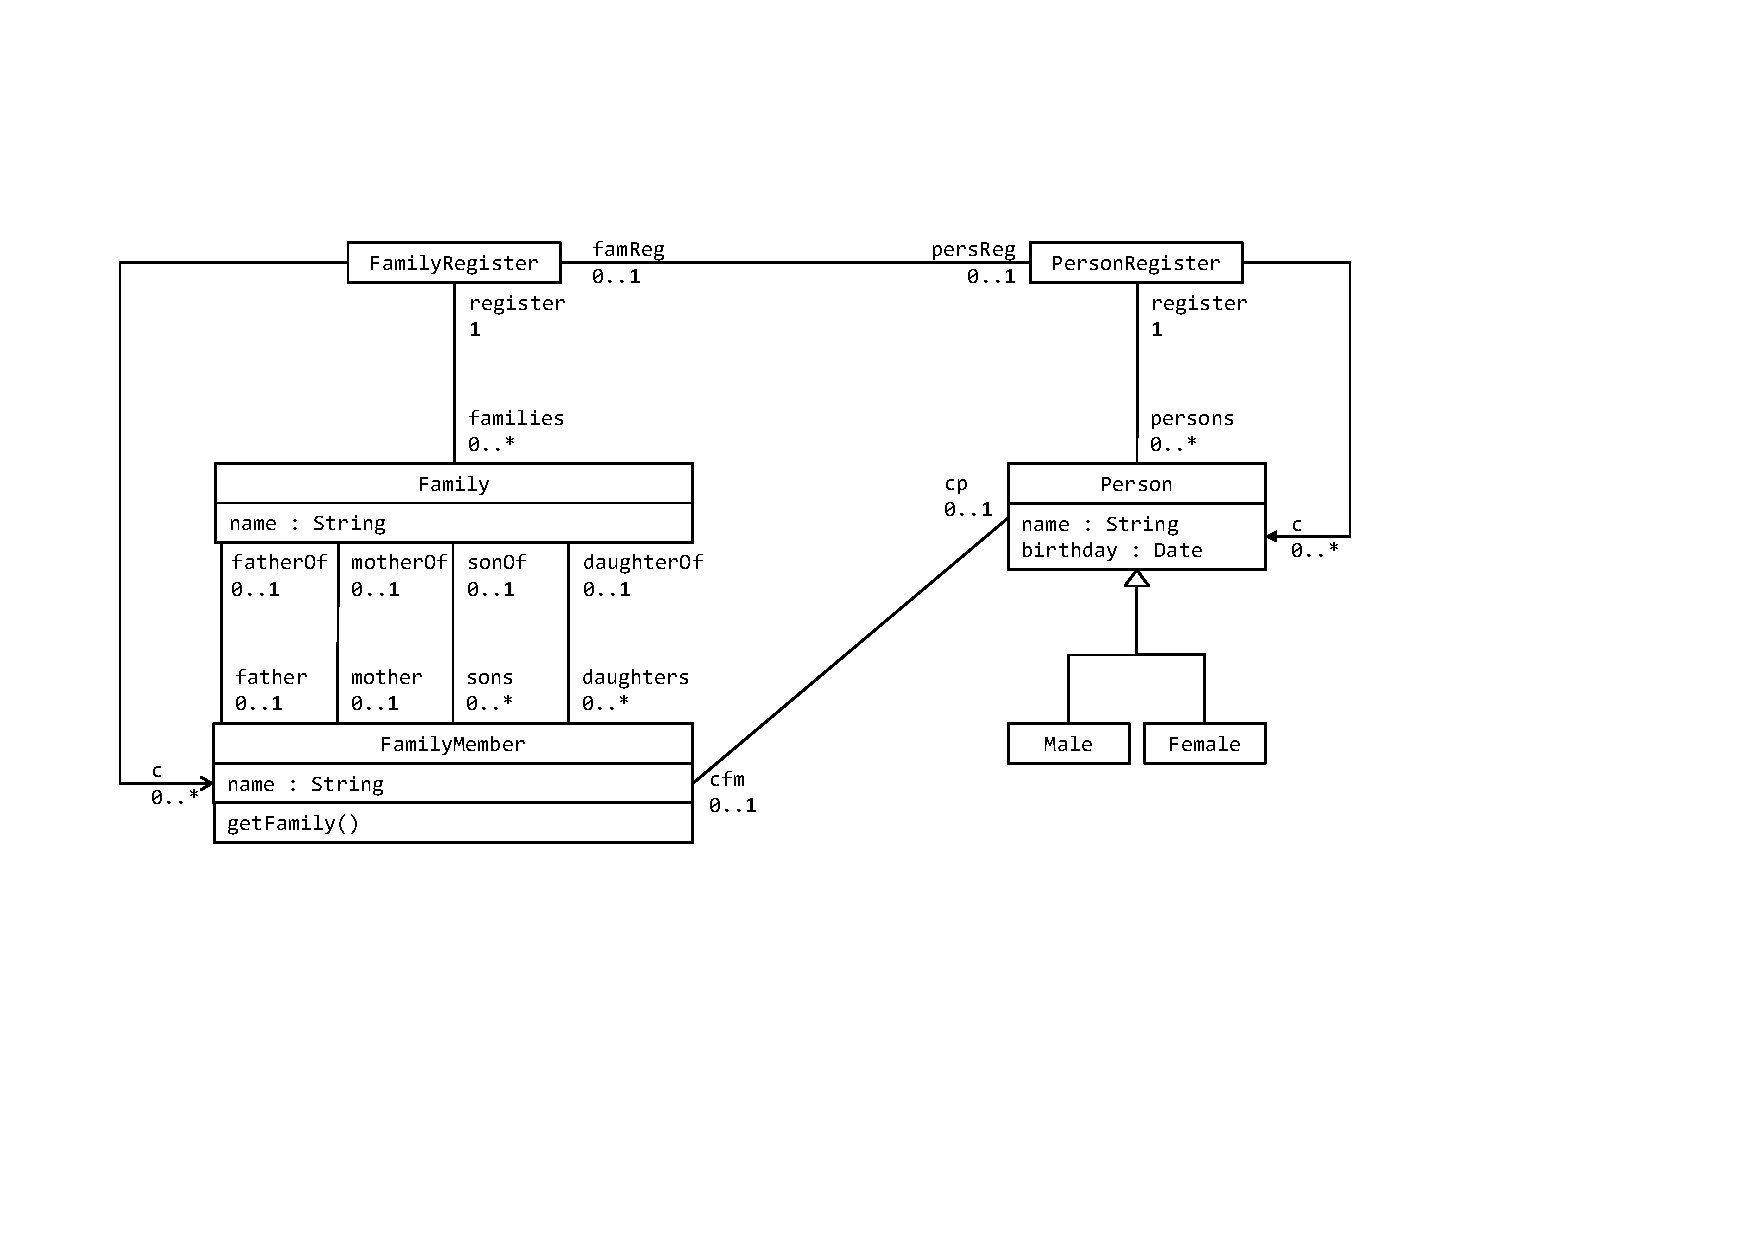
\includegraphics[width=0.75\textwidth]{diagrams/solutions/SDMLibModel}
	\caption{SDMLib model used for the benchmark}
	\label{fig:SDMLibModel}
\end{figure*}

\subsection{SDMLib}
\label{sec:SDMLib}

SDMLib, short for \emph{Story Driven Modeling Library}\footnote{http://www.sdmlib.org}, is a Java library to support Story Driven Modeling~\cite{Norbisrath2013}, a formalism based on graph transformations~\cite{Ehrig2006}.
SDMLib provides an internal DSL with Java as a host language.
Although SDMLib is not a bx tool, in the sense that it does not provide any extra support especially for developing bx, it is nonetheless included here as a ``general purpose'' model transformation tool against which bx tools should also be compared. 

As models can be viewed as attributed, typed \emph{graphs}, model transformations can also be regarded as a problem in the domain of graph transformations.
A \emph{graph rewrite rule} specifies the replacement of a graph pattern (left-hand side) by a subgraph to be embedded into the overall host graph.
Graph rewrite rules can be used to specify not only in-place model transformations, but also 
model-to-model transformations by applying the rules to multiple graphs.
Graph rewrite rules are \emph{declarative} in the sense that the exact order in which to traverse the host graph and check for or replace patterns is not specified.


\subsubsection{Classification}
The solution to the benchmark with SDMLib follows a \emph{restoration-based} architectural style; \emph{fCR} and \emph{bCR} are implemented with graph rewrite rules. 

The solution addresses the \emph{initial-diag-based} application scenario (figure \ref{fig:initialDiagBased}).
A diag is taken as input, and the dependent model is manipulated until both models are consistent again. 

No formal guarantees are provided by SDMLib as \emph{fCR} and \emph{bCR} are specified separately and independently.
It is left up to the transformation developer to ensure that the implementations are not contradictory.
As with the BXtend solution, this can be viewed as an advantage; the bx programmer may freely decide whatever is necessary to solve the current task.

The SDMLib solution has no explicit notion of \emph{consistency} as it is \emph{implicitly} given by the implemented pair of \emph{fCR/bCR}.
Accordingly, synchronization \emph{control} is \emph{explicit}, and programmed by providing suitable graph rewrite rules.
The SDMLib solution was developed with the benchmark in mind and thus supports \emph{directed}, \emph{on demand}, \emph{automatic} synchronization. 

\subsubsection{Benchmark solution with SDMLib}

The following description is based on the SDMLib solution for the Families-to-Persons benchmark at TTC 2017~\cite{Zundorf2017}.
As SDMLib is designed for in-place transformations on a single host graph, the solution uses a single metamodel as depicted in figure~\ref{fig:SDMLibModel}.
To support incrementality efficiently, additional unidirectional references between \code{FamilyRegister} and \code{Fami\-lyMember}, and \code{PersonRegister} and \code{Person} are used to detect changed elements.
Finally, the correspondences are represented using two bidirectional references.
The SDMLib solution thus operates on a single graph comprising the contents of both models as well as explicit correspondence links between respective elements. 

\begin{lstlisting}[label={lst:sdmlib}, float=hbt!, language=java, caption={Forward transformation in SDMLib}]
private void transformForward() {
 familyRegisterPO = new FamilyRegisterPO()
   .withPatternObjectName("fr");
 PersonRegisterPO personRegisterPO = 
  familyRegisterPO.createPersonRegisterPO()
                  .withPatternObjectName("pr");
 FamilyMemberPO memberPO = familyRegisterPO
   .createCPO()
   .withPatternObjectName("fm");

 // there is an old corresponding person
 memberPO.startSubPattern();
 PersonPO oldPersonPO = memberPO.createCpPO()
   .withName("oldP");
 oldPersonPO.createCondition(p -> 
   ensureNameAndGender(p));
 memberPO.endSubPattern();

 // no corresponding person
 memberPO.startNAC();
 memberPO.createCpPO()
   .withPatternObjectName("noOldP");
 memberPO.endNAC();
 MalePO personPO = memberPO
   .createCpMalePO(Pattern.CREATE)
   .withPatternObjectName("newP");
 personPO.createRegisterLink(
   personRegisterPO, 
   Pattern.CREATE);
 personPO.createCondition(p -> 
   ensureNameAndGender(p));
    
 familyRegisterPO.createLink(
   memberPO, 
   Pattern.DESTROY);

 familyRegisterPO.rebind(familyRegister);
 familyRegisterPO.doAllMatches();	    
}
\end{lstlisting}

The core of the SDMLib solution consists of two graph rewrite rules, one for each direction.
While graph rewrite rules are typically presented using a visual concrete syntax, we use the actual textual concrete syntax provided by the tool to enable and simplify a comparison with all other solutions.  

Listing~\ref{lst:sdmlib} depicts the graph rewrite rule for the forward transformation using SDMLib's internal DSL, embedded into Java.
The method for the graph rewrite rule uses code generated from the graph metamodel depicted in figure~\ref{fig:SDMLibModel}. 

The statements on line~2--9 define story pattern objects for the family register, the person register, and a family member, which need to be matched in the families model; the links connecting these objects are added implicitly to the story pattern by the invoked methods (e.g., \code{createCPO()}). 

Lines~12-17 handle the case that a corresponding person object already exists.
This case is realized with an optional subpattern, which is started at line~12 and is terminated at line~17.
The pattern is composed of an old person object, connected to the family member object by a correspondence link.
If pattern matching succeeds, the method \code{ensure\-Name\-And\-Gender} is invoked to restore consistency.

Lines~20--31 deal with the case where there is no corresponding person object.
This is handled with a \emph{negative application condition}, defined on lines~20--23.
On lines~17--19, elements of story patterns are created that define the actions to be performed when the negative application condition holds: A person object has to be created and linked to the person register; the method \code{ensure\-Name\-And\-Gender} is then called to establish consistency with the family object.

Finally, the temporary link between the family register and the family member --- which is set in the course of changes to the families model --- is matched and then removed (lines~33--35), the story pattern object for the family register is bound (line~37), and the pattern is applied to all matches (line~38).

%%% Local Variables:
%%% mode: latex
%%% TeX-master: "../main"
%%% End:
